
\documentclass[final]{beamer}

\usepackage[scale=1.24]{beamerposter} % Use the beamerposter package for laying out the poster
\usetheme{confposter} % Use the confposter theme supplied with this template

\usepackage[
    backend=biber,
    style=nature,
    sortlocale=de_DE,
    url=false,
    doi=true,
    eprint=false,
    citestyle=numeric
]{biblatex}
\addbibresource{reference.bib}


\setbeamercolor{block title}{fg=dblue,bg=white} % Colors of the block titles
\setbeamercolor{block body}{fg=black,bg=white} % Colors of the body of blocks
\setbeamercolor{block alerted title}{fg=white,bg=dblue!70} % Colors of the highlighted block titles
\setbeamercolor{block alerted body}{fg=black,bg=dblue!10} % Colors of the body of highlighted blocks
% Many more colors are available for use in beamerthemeconfposter.sty

%-----------------------------------------------------------
% Define the column widths and overall poster size
% To set effective sepwid, onecolwid and twocolwid values, first choose how many columns you want and how much separation you want between columns
% In this template, the separation width chosen is 0.024 of the paper width and a 4-column layout
% onecolwid should therefore be (1-(# of columns+1)*sepwid)/# of columns e.g. (1-(4+1)*0.024)/4 = 0.22
% Set twocolwid to be (2*onecolwid)+sepwid = 0.464
% Set threecolwid to be (3*onecolwid)+2*sepwid = 0.708

\newlength{\sepwid}
\newlength{\onecolwid}
\newlength{\twocolwid}
\newlength{\threecolwid}
\setlength{\paperwidth}{48in} % A0 width: 46.8in
\setlength{\paperheight}{36in} % A0 height: 33.1in
\setlength{\sepwid}{0.024\paperwidth} % Separation width (white space) between columns
\setlength{\onecolwid}{0.22\paperwidth} % Width of one column
\setlength{\twocolwid}{0.464\paperwidth} % Width of two columns
\setlength{\threecolwid}{0.708\paperwidth} % Width of three columns
\setlength{\topmargin}{-0.5in} % Reduce the top margin size
%-----------------------------------------------------------

\usepackage{graphicx}  % Required for including images
\graphicspath{ {../manuscript/figures/} }
% \graphicspath{ {figures/} }


\usepackage{booktabs} % Top and bottom rules for tables

%----------------------------------------------------------------------------------------
%	TITLE SECTION
%----------------------------------------------------------------------------------------

\title{Ki-67 Digital Image Analysis: Reliability and Variability} % Poster title

\author{\normalsize{Peiqi Wang$^1$, Tian Yu Liu$^2$, Willa Shi$^3$, Sehrish Butt$^4$, Trevor McKee$^4$, Fei-Fei Liu$^{1,3}$, Naomi A. Miller$^3$, Adewunmi Adeoye$^3$, David McCready$^3$, Anthony Fyles$^3$, Susan J. Done$^{1,3}$}} % Author(s)

\institute{\small{$1.$ Department of Medical Biophysics, University of Toronto, Canada; $2.$ Faculty of Music, University of Toronto, ON, Canada; $3.$ Princess Margaret Cancer Centre, Canada; $4.$ STTARR Medical Diagnostics Imaging Center}} % Institution(s)


%----------------------------------------------------------------------------------------

\begin{document}
\renewcommand{\baselinestretch}{0.6}
\addtobeamertemplate{block end}{}{\vspace*{2ex}} % White space under blocks
\addtobeamertemplate{block alerted end}{}{\vspace*{2ex}} % White space under highlighted (alert) blocks

\setlength{\belowcaptionskip}{2ex} % White space under figures
\setlength\belowdisplayshortskip{2ex} % White space under equations

\begin{frame}[t] % The whole poster is enclosed in one beamer frame

\begin{columns}[t] % The whole poster consists of three major columns, the second of which is split into two columns twice - the [t] option aligns each column's content to the top

\begin{column}{\sepwid}\end{column} % Empty spacer column
%
\begin{column}{\onecolwid} % The first column

%----------------------------------------------------------------------------------------
%	Abstract
%----------------------------------------------------------------------------------------

\begin{block}{Abstract}
\begin{itemize}
\item In this study, we evaluated two digital image analysis (DIA) methods - Aperio ePathology and Definiens Tissue Studio
\item  We assessed reliability of the two DIA methods by reporting their agreement to a set of manual scores previously identified to be a predictor of ipsilateral breast cancer relapse in the the Toronto-British Columbia (TBC) trial patient cohort
\item We compared agreements within and between the DIA methods so as to evaluate intra- and inter-algorithmic variability.
\item We also discussed potential sources of variability and ways to mitigate them
\end{itemize}
\end{block}

% ----------------------------------------------------------------------------------------
% 	Background
% ----------------------------------------------------------------------------------------

\begin{block}{Background}
\begin{itemize}
\item Ki-67 is a human nuclear protein detected exclusively in the active phases of the cell cycle, namely $G_1$, $S$, $G_2$, and mitosis, while absent in the resting $G_0$ phase.\cite{Gerdes1984}
\item A multitude of studies report the use of Ki-67 labeling index in predicting disease free/overall survival and tumour recurrence \cite{Stuart-Harris2005} as well as in guiding neoadjuvant chemotherapy. \cite{Jones2009}
\item Despite its apparent value in cancer prognosis, widespread use of Ki-67 labeling index in clinical pathology is hampered by the lack of standardization and suffers from substantial intra- and interobserver variability. \cite{Dowsett2011a, Polley2013a}
\item DIA ensures automaticity, repeatability and reproducibility.
\item In addition to validate its reliability by comparing with traditional manual assessment methods, there is a great need to validate the reliability of existent Ki-67 DIA methods so as to identify major sources of variability and potential solutions.
\end{itemize}
\end{block}


\begin{block}{Methods}
{\bf Manual Assessment}
\newline

A trained individual, assigned as rater 1, counted at least 200 cells within tumour hot spot, or areas in which Ki-67 most frequently expressed, for each core, and Ki-67 labeling index is calculated
\newline

{\bf Digital Image Analysis (DIA)}
\newline

2 trained individuals, assigned as rater 1 and rater 2, independently marked tumour region of interest (ROI) for proper image segmentation in the Aperio system. The same set of images were analyzed using the Definiens system. In this case, a technician, assigned as rater 3, segmented images in a few cases, which calibrated the software to perform semi-automatic segmentation.
\end{block}

\end{column} % End of the first column
%
%
\begin{column}{\onecolwid} % The first column
%
% %----------------------------------------------------------------------------------------
% %	MATERIALS
% %----------------------------------------------------------------------------------------

\begin{block}{}

{\bf Statistics}
\newline

Data distribution for different scoring methods were visualized using boxplot, accompanied by summary statistics. Bland-Altman plot was used to visualize agreements between results from two DIA methods in relation to manual score reference. Concordance between methods was quantified using a two-way mixed, average-measures intraclass correlation coefficient (ICC). Conger generalized Kappa ($\kappa$) were calculated based on a set of commonly used cut-offs for Ki-67 positivity to evaluate the practicality of consistent classification using results from methods tested.


\begin{figure}
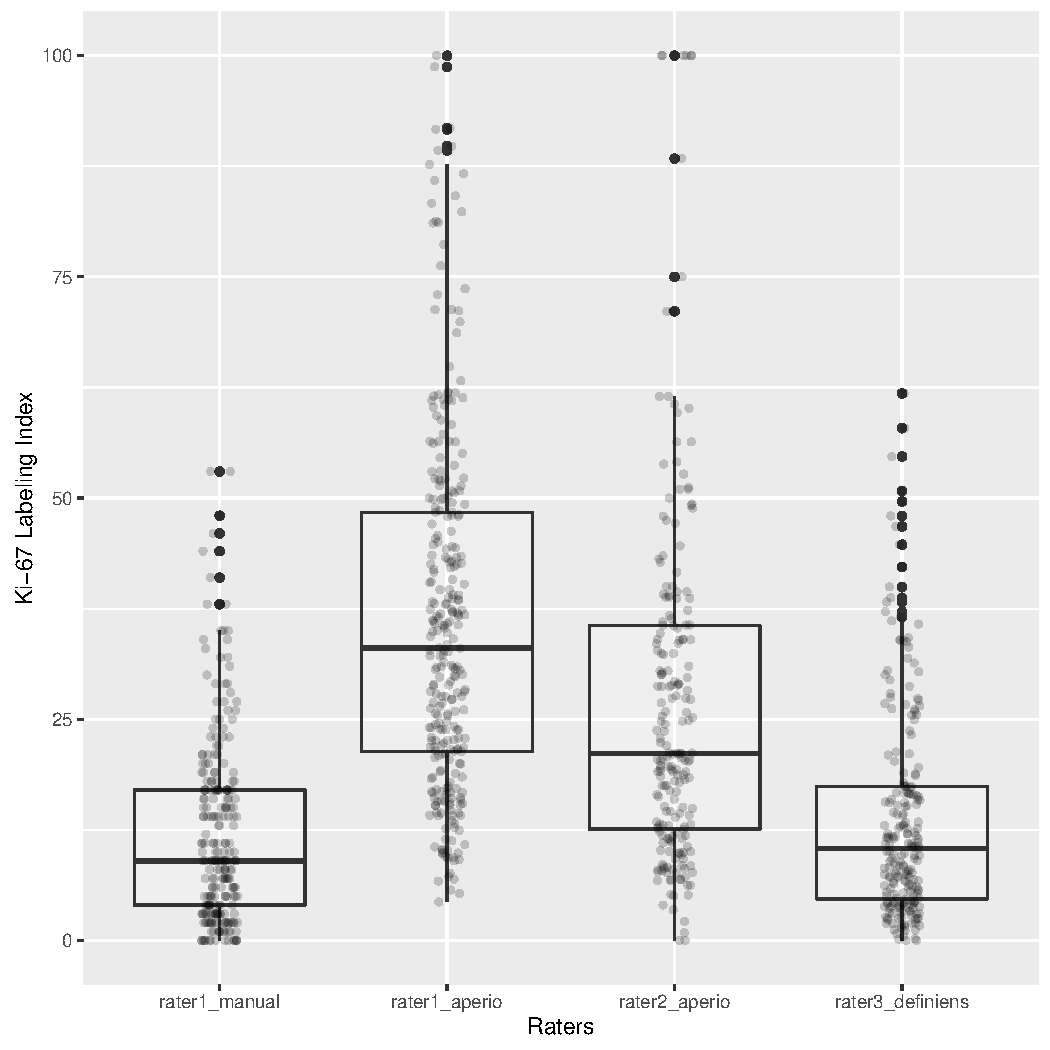
\includegraphics[width = 0.4\linewidth]{boxplot}
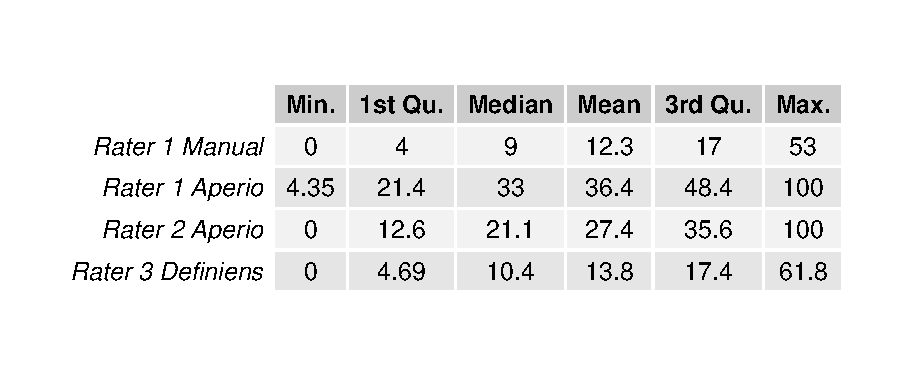
\includegraphics[width = 0.6\linewidth]{boxStat}

\centering
\caption{
{\bf Boxplot and summary statistics}
Distribution of Ki-67 labeling index generated using manual assessment and DIA methods. Outliers are represented as darkened circles. Corresponding summary statistics quantitatively descibes the boxplot.
}
\label{boxplot}
\end{figure}
\end{block}


\begin{block}{Results}
\newline

{\bf Overall Distribution}
\newline

Boxplot of untransformed Ki-67 labeling index as well as summary statistics are presented in Figure~\ref{boxplot}. The Aperio system tended to overestimate Ki-67 labeling index; whereas the Definiens system showed a similar distribution to manual score reference.
\newline

{\bf Agreement to Manual Score Reference} \newline

Bland-Altman plot for every DIA method compared to manual score reference and relevant statistics are presented in Figure~\ref{baplot}. The Aperio system systematically overestimated Ki-67 labeling index by a large margin in both scoring instances. The Definiens system faired better in introducing minimal bias, but still exhibited non-negligible variability.

ICC comparing two rating instances using the Aperio system and the manual score reference were 0.173 (95\%CI -0.245 $\sim$ 0.459) and 0.439 (95\%CI -0.258 $\sim$  0.72) respectively, representing poor to moderate agreements. ICC comparing the Definiens system and the manual score reference was 0.892 (95\%CI 0.841 $\sim$ 0.924), indicating high degree of agreement. The Ki-67 labeling index was scored similarly using manual assessment and the Definiens system.

\end{block}

\end{column}


\begin{column}{\onecolwid} % The first column

\begin{block}{}

It may be misleading to solely measure absolute agreement, as ultimately cases would be classified into clinically relevant groups based on the Ki-67 labeling index. Kappa statistics calculated using cut-offs from a meta-analysis study were listed in Figure~\ref{kappaStat}. With a 14\% cut-off used to distinguish luminal B from luminal A tumours,  $\kappa$ obtained using the Definiens system was 0.67, suggesting a substantial agreement in making clinically relevant classifications.


\begin{figure}
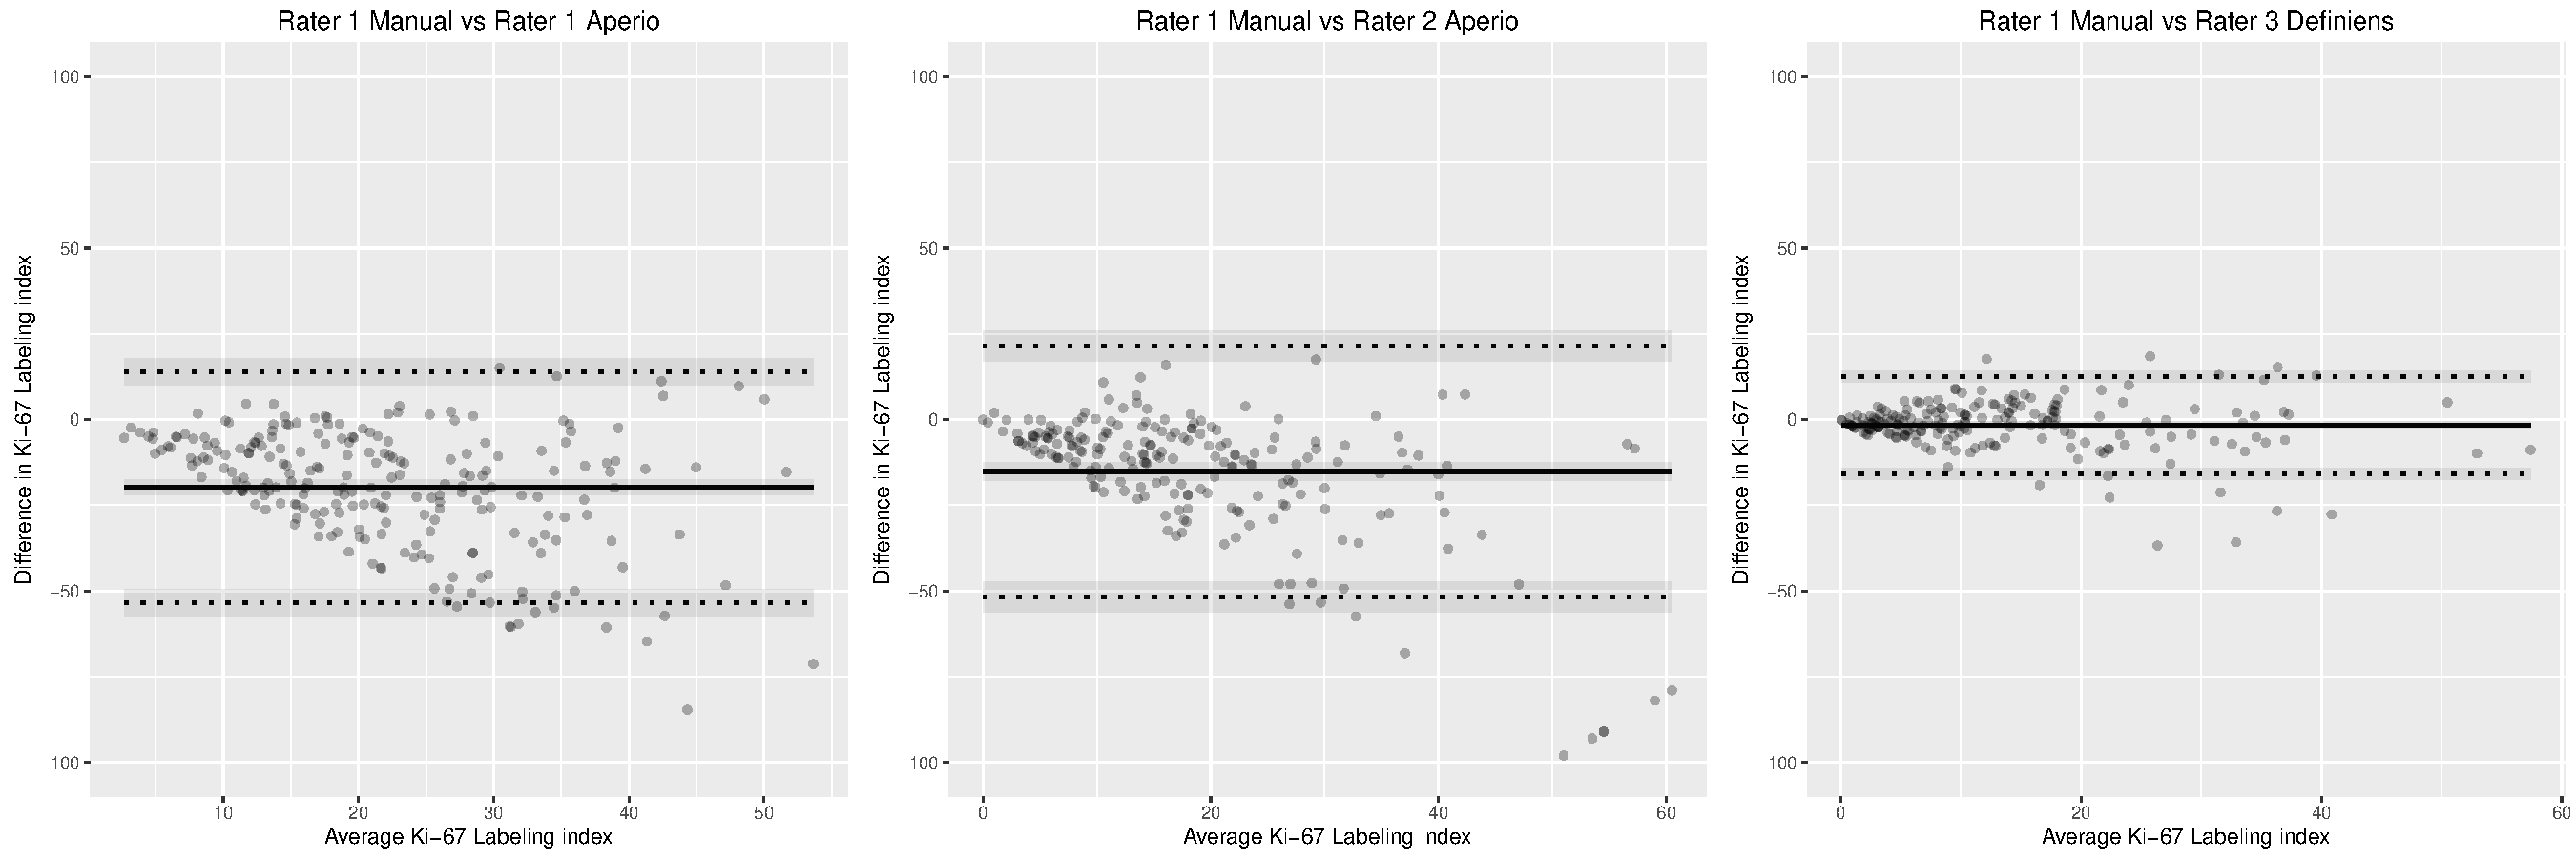
\includegraphics[width = \linewidth]{baplot}
\end{figure}

\begin{figure}
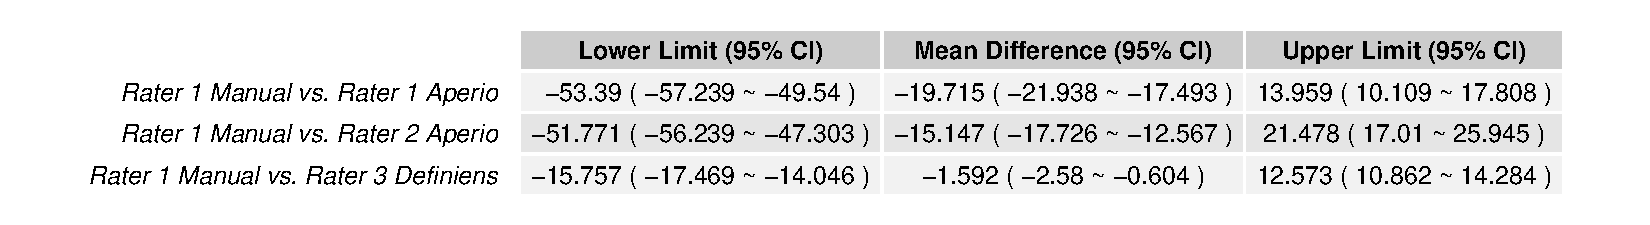
\includegraphics[width = \linewidth]{baStat}

\centering
\caption{{\bf Bland-Altman Plot}
Bias and agreement interval of manual reference score compared to results from DIA methods. Bland-Altman plot consists of a scatterplot, with each data point representing paired Ki-67 labeling index generated using methods in comparison. X axis is the average of paired measurement while the Y axis is the difference of paired measurement. Data points are flanked by dashed lines, which represent limits of agreement, within which 95\% of differences fall. Confidence intervals of mean difference as well as upper and lower limit of agreement are shown as grey area surrounding them. Statistics relevant to the plot are tabulated in the accompanying table.
}
\label{baplot}
\end{figure}


{\bf High Intra- and Inter-algorithmic Variability}
\newline

ICC between two rating instances when using the Aperio system was 0.538 (95\%CI: 0.31 $\sim$ 0.68), which represented moderate agreement. Additionally, $\kappa$ comparing two rating instances using the Aperio system indicated slight to fair agreement as presented in Figure~\ref{kappaStat}. As the same analytical settings were used for both rating instances, manual image segmentation was responsible for the differences in Ki-67 labeling index generated. A substantial amount of variability was introduced in the process of image segmentation.


ICC comparing 2 rating instances using the Aperio system and the Definiens system were 0.351 (95\%CI: -0.315 $\sim$ 0.678) and 0.596 (95\%CI: -0.182 $\sim$ 0.823). $\kappa$ comparing the two DIA methods was slight to fair as presented in Figure~\ref{kappaStat}. High inter-algorithmic variability was observed between the two DIA methods. It was difficult to control for differences when using the two DIA methods. However, algorithm implementation, segmentation procedure, and rater bias all contribute to perceived high inter-algorithmic variability.






\end{block}
\end{column}


\begin{column}{\onecolwid}

\begin{block}{}

\begin{figure}
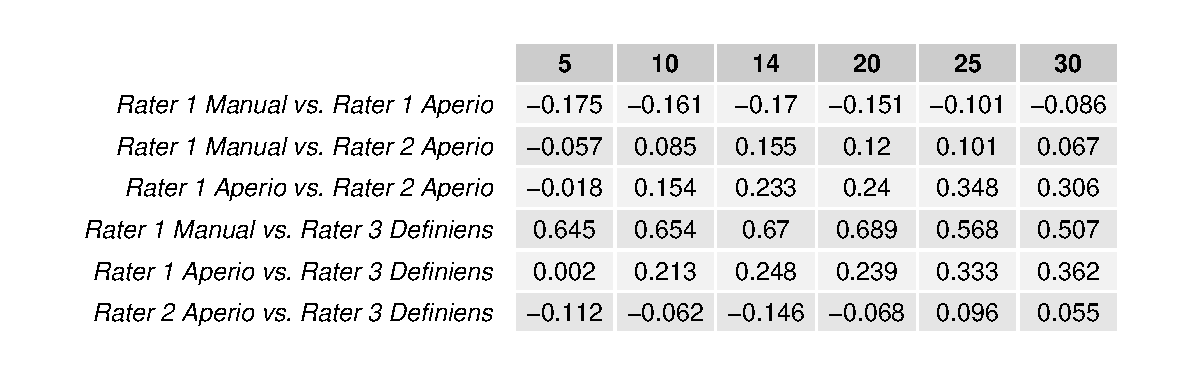
\includegraphics[width = \linewidth]{kappaStat}
\centering
\caption{
{\bf Kappa statistics}
$\kappa$ calculated is a measurement of the extent that different rating instances correctly classify Ki-67 labeling index into Ki-67 low and Ki-67 high based on a selection of cut-offs, namely 5\%, 10\%, 14\%, 20\%, 25\%, 30\%.
}
\label{kappaStat}
\end{figure}

\end{block}


\begin{block}{Conclusion}

\begin{itemize}
\item In this study, we assessed agreements of results from two DIA methods to a set of manual score reference (n=278) that is prognostically relevant. The Definiens system was observed to agree well with the manual score reference, both in absolute value of Ki-67 labeling index and in its ability to segregate cases into clinically relevant groups.
\item Although DIA can be highly accurate, not all DIA methods have a good performance.
\item High intra- and inter-algorithmic variability was observed when the two DIA methods were compared within and between themselves.
\item We identified image segmentation as a hugely important contributor to high intra-algorithmic variability in the Aperio system, when all else is kept consistent.
\item Additionally, systematic bias was detrimental toward achieving high agreement. In our study, we identified settings assignments as potential major source of such discrepancy, in addition to different algorithm implementations.
\end{itemize}

In conclusion, DIA method can perform comparably with traditional manual assessment methods. Intra- and inter-algorithmic variability is considerable amongst the two DIA methods tested and can be a prevalent phenomenon, hindering valid comparison across different DIA platforms. Settings assignments and image segmentation are major sources of such variability. Novel algorithms on calibration and segmentation are needed toward standardized DIA procedure.

\end{block}


\begin{block}{References}
\renewcommand*{\bibfont}{\tiny}
\printbibliography
\end{block}

\end{column}


\end{columns} % End of all the columns in the poster

\end{frame} % End of the enclosing frame

\end{document}
